\documentclass{standalone}
\usepackage{tikz}

\begin{document}
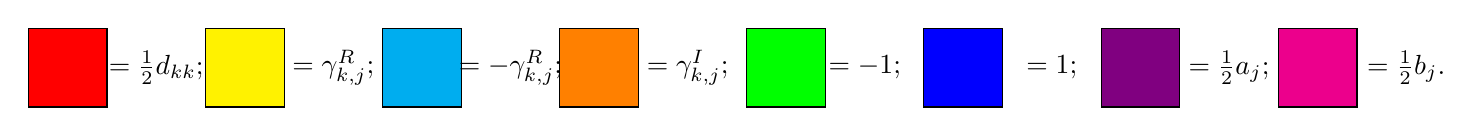
\begin{tikzpicture}
\draw [fill=red] (0,0) rectangle (1,-1);
\node at (1.625,-0.5) {$=\frac{1}{2} d_{kk}$;};
\draw [fill=yellow] (2.25,0) rectangle (3.25,-1);
\node at (3.875,-0.5) {$=\gamma_{k,j}^{R}$;};
\draw [fill=cyan] (4.5,0) rectangle (5.5,-1);
\node at (6.125,-0.5) {$=-\gamma_{k,j}^{R}$;};
\draw [fill=orange] (6.75,0) rectangle (7.75,-1);
\node at (8.375,-0.5) {$=\gamma_{k,j}^{I}$;};
\draw [fill=green] (9.125,0) rectangle (10.125,-1);
\node at (10.625,-0.5) {$= -1$;};
\draw [fill=blue] (11.375,0) rectangle (12.375,-1);
\node at (13.,-0.5) {$= 1$;};
\draw [fill=violet] (13.625,0) rectangle (14.625,-1);
\node at (15.25,-0.5) {$=\frac{1}{2}a_j$;};
\draw [fill=magenta] (15.875,0) rectangle (16.875,-1);
\node at (17.5,-0.5) {$=\frac{1}{2}b_j$.};
\end{tikzpicture}
\end{document}
